\documentclass[aspectratio=43]{beamer}
% Theme works only with a 4:3 aspect ratio
\usetheme{CSCS}

\usepackage{tikz}
\usepackage{mwe}
\usepackage{pgfplots}
\usepackage{pgfplotstable}
\usetikzlibrary{pgfplots.groupplots,spy,patterns}
\usetikzlibrary{arrows.meta}
\usetikzlibrary{positioning}
\usepackage{listings}
\usepackage{color}
\usepackage{tcolorbox}
\usepackage{anyfontsize}
\usepackage{xspace}
\usepackage{graphicx}
\usepackage{pifont}
\usepackage{lstautogobble}

\definecolor{reallylightgray}{rgb}{0.95,0.95,0.95}
\definecolor{darkgreen}{rgb}{0.0,0.5,0.0}

% define footer text
\newcommand{\footlinetext}{Arbor: a neuroscience library for HPC}

% Select the image for the title page
\newcommand{\picturetitle}{cscs_images/image5.pdf}

% fonts for maths
\usefonttheme{professionalfonts}
\usefonttheme{serif}

% source code listing
\newcommand\TS{\rule{0pt}{2.6ex}}       % Top strut
\newcommand\BS{\rule[-1.2ex]{0pt}{0pt}} % Bottom strut
\newcommand{\hl}[1]{\textbf{\textcolor{blue}{#1}}} % for hilighting optimal entries in tables
\newcommand{\rl}[1]{\textbf{\textcolor{red}{#1}}} % for hilighting sub-optimal entries in tables
\newcommand{\img}[1]{{\Large \textbf{IMAGE {#1}}}}
\newcommand{\hilight}[1]{\textcolor{blue!20!orange}{#1}}
\newcommand{\arbor}{{\ttfamily Arbor}\xspace}
\newcommand{\neuron}{{\ttfamily NEURON}\xspace}
\newcommand{\coreneuron}{{\ttfamily CoreNeuron}\xspace}
\newcommand{\daintmc}[0]{Daint-mc\xspace}
\newcommand{\daintgpu}[0]{Daint-gpu\xspace}
\newcommand{\tave}[0]{Tave-knl\xspace}
\newcommand{\pder}[2]{\frac{\partial{#1}}{\partial{#2}}}
\newcommand*\mytitle{\fontsize{14.5}{16}\selectfont}

% set indent to a more reasonable level (so that itemize can be used in columns)
\setlength{\leftmargin}{20pt}

\DeclareTextFontCommand{\emph}{\color{blue!85!black}}

\author{\textbf{Nora Abi Akar}, Ben Cumming, Stuart Yates, Thorsten Hater, Brent Huisman, Anne K\"usters.}
\title{\mytitle \arbor: a simulation library designed for HPC}
\subtitle{PASC21}

\begin{document}

% TITLE SLIDE
\cscstitle

%-------------------------------------------
\begin{frame}[fragile]{\arbor}
    \arbor is a library for the simulation of morphologically-detailed neuronal networks on HPC systems.
    \begin{itemize}
        \item \emph{key aim}: enabling simulation on all HPC systems.
        \item \emph{key aim}: providing rich interfaces and enabling diverse use cases.
    \end{itemize}

    \vspace{10pt}
    \emph{All features} are implemented and optimised on \emph{all platforms}
    \begin{itemize}
        \item GPUs (CUDA, Clang-CUDA, HIP)
        \item SIMD CPU backends: (AVX, AVX2, AVX512, Neon, SVE).
        \item Distributed simulation (MPI).
    \end{itemize}
    \vspace{10pt}

    %Requires a \emph{rich interface} for defining models.
    %\begin{itemize}
    %    \item Simulation of electrical current in arbitrarily complex morphologies.
    %    \item Arbitrary ion channel and synapse models.
    %    \item Inter-cell communication via spikes on arbitrary networks.
    %\end{itemize}
\end{frame}
%-------------------------------------------

%-------------------------------------------
\begin{frame}[fragile]{Models are varied and complicated}
    \begin{center}
        \includegraphics[width=0.35\textwidth]{images/purkinje_cell.png}
        \\
        {
            \tiny Drawing of a Purkinje cell in the cerebellar cortex by Santiago Ram\`{o}n y Caja.
        }
    \end{center}
    Arbor is designed to simulate \textbf{millions} of these cells and their interactions.
\end{frame}
%-------------------------------------------

%-------------------------------------------
\begin{frame}[fragile]{\arbor weak scaling}
    \begin{figure}[htp!]
       \begin{center}
           \begin{tikzpicture}
    [scale=0.9, every node/.style={scale=0.9}]
    \begin{axis}[
        %axis y discontinuity=crunch,
        xmode=log,
        height=0.5\textwidth,
        width=1\textwidth,
        xmin=1,xmax=128,
        ymin=80, ymax=90,
        %ytick={60,70,80,90,100},
        %yticklabels={,70,80,90,100},
        xtick={1, 2, 4, 8 , 16, 32, 64, 128},
        xticklabels={1, 2, 4, 8 , 16, 32, 64, 128},
        ylabel=wall time (s),
        xlabel=nodes,
        %axis y line*=left,
        xticklabel style={yshift=-2pt},
        yticklabel style={xshift=-2pt},
        legend style = {at={(1,0)}, anchor=south east},
        line width=1pt,
        every axis y label/.style=
            {at={(ticklabel cs:0.5)},rotate=90,anchor=near ticklabel},
        grid=major]

        \addplot[color=blue, mark=*, mark size=1.5, mark options={fill=white}]
            table[x=nodes,y=mc_wall] {./data/weak_real.tbl};
        \addplot[color=red, mark=*, mark size=1.5, mark options={fill=white}]
            table[x=nodes,y=gpu_wall] {./data/weak_real.tbl};

       \legend{ {\scriptsize \daintmc},
                {\scriptsize \daintgpu},
              };
    \end{axis}
\end{tikzpicture}

           \caption{
               Simulation time for the \textbf{weak} scaling tests with 8,192 cells per node, 1 to 128 nodes (8192 to 1,048,576 cells).
               Each cells is connected to 10,000 random cells with no self-connections.
           }
           \label{fig:weak_tts}
       \end{center}
    \end{figure}
\end{frame}
%-------------------------------------------

%-------------------------------------------
\begin{frame}[fragile]{\arbor strong scaling}
    \begin{figure}[htp!]
        \centering
        \begin{tikzpicture}
    [scale=0.62, every node/.style={scale=0.62}]
    \begin{axis}[
        xmode=log,
        height=0.52\textwidth,
        width=0.8\textwidth,
        xmin=1, xmax=64,
        xtick={1, 2, 4, 8, 16, 32, 64},
        xticklabels={1, 2, 4, 8, 16, 32, 64},
        ymin=0.0, ymax=1.05,
        ytick={0, 0.1, 0.2, 0.3, 0.4, 0.5, 0.6, 0.7, 0.8, 0.9, 1},
        yticklabels={0, 10, 20, 30, 40, 50, 60, 70, 80, 90, 100},
        ylabel=strong scaling efficiency (\%),
        xlabel=nodes,
        xticklabel style={yshift=-2pt},
        yticklabel style={xshift=-2pt},
        legend style = {at={(0,0)}, anchor=south west},
        line width=1pt,
        every axis y label/.style=
            {at={(ticklabel cs:0.5)},rotate=90,anchor=near ticklabel},
        grid=major]

        \addplot[color=green]
            table[x=nodes,y=p_eff] {data/strong_multi.tbl};
        \addplot[color=blue, mark=*, mark size=2, mark options={fill=white}]
            table[x=nodes,y=mc_eff] {data/strong_multi.tbl};
        \addplot[color=red, mark=triangle, mark size=2, mark options={fill=white}]
            table[x=nodes,y=gpu_eff] {data/strong_multi.tbl};
        \addplot[color=orange, mark=square, mark size=2, mark options={fill=white}]
            table[x=nodes,y=knl_eff] {data/strong_multi.tbl};

       \legend{ {\scriptsize perfect},
                {\scriptsize \daintmc},
                {\scriptsize \daintgpu},
                {\scriptsize \tave},
              };
    \end{axis}
    \end{tikzpicture}

        \begin{tikzpicture}
    [scale=0.62, every node/.style={scale=0.62}, font=\large]
    \begin{axis}[
        xmode=log,
        height=0.52\textwidth,
        width=0.8\textwidth,
        xmin=1, xmax=64,
        xtick={1, 2, 4, 8, 16, 32, 64},
        xticklabels={1, 2, 4, 8, 16, 32, 64},
        ymin=100, ymax=400,
        %ytick={30,40,50,60,70,80},
        ylabel=node seconds (ns),
        xlabel=nodes,
        xticklabel style={yshift=-2pt},
        yticklabel style={xshift=-2pt},
        line width=1pt,
        every axis y label/.style=
            {at={(ticklabel cs:0.5)},rotate=90,anchor=near ticklabel},
        grid=major]

        \addplot[color=blue, mark=*, mark size=2, mark options={fill=white}]
            table[x=nodes,y expr=\thisrow{mc_time}*\thisrow{nodes}] {data/strong_multi.tbl};
        \addplot[color=red, mark=triangle, mark size=2, mark options={fill=white}]
            table[x=nodes,y expr=\thisrow{gpu_time}*\thisrow{nodes}] {data/strong_multi.tbl};
        \addplot[color=orange, mark=square, mark size=2, mark options={fill=white}]
            table[x=nodes,y expr=\thisrow{knl_time}*\thisrow{nodes}] {data/strong_multi.tbl};

    \end{axis}
\end{tikzpicture}

        \caption{
            \textbf{Strong} scaling from 1 to 64 nodes of a 100~ms simulation with 16,384 cells and 10,000 randomly connected synapses.
        }
        \label{fig:strong_multi}
    \end{figure}
\end{frame}
%-------------------------------------------

%-------------------------------------------
\begin{frame}[fragile]{\arbor design requirements}
    This talk will focus on the \textbf{guiding design principles} of \arbor:
    \begin{itemize}
        \item \emph{Portability}
        \begin{itemize}
            \item Model portability.
            \item Performance portability.
        \end{itemize}
        \item \emph{Scalability}
        \begin{itemize}
            \item Distributed model construction.
            \item Efficient communication schemes. 
        \end{itemize}
        \item \emph{Extensibility}
        \begin{itemize}
            \item New hardware. 
            \item New numerical solvers ... 
        \end{itemize}
    \end{itemize}
\end{frame}
%-------------------------------------------

%-------------------------------------------
\cscschapter{1. Portability}
%-------------------------------------------

%-------------------------------------------
\begin{frame}[fragile]{Model portability}
    One of the main challenges has been defining an interface for inputting models.
    
    \begin{itemize}
        \item Model descriptions should be simulator and architecture agnostic.
        \item This requires \emph{separation of concerns} between model description and implementation.
    \end{itemize}

    \vspace{10pt}

    \arbor supports portable descriptions by:
    \begin{enumerate}
        \item Using flat model descriptions: describe \emph{what, not how}.
        \item Separating hardware and implementation details from model description interface.
    \end{enumerate}

\end{frame}
%-------------------------------------------

%-------------------------------------------
\begin{frame}[fragile]{Model portability}
    \emph{What}: model description: 
    \begin{itemize}
        \item Flat descriptions of individual cells. 
        \item Flat description of the network.
    \end{itemize}

    \vspace{10pt}

    \emph{How}: model implementation: 
    \begin{itemize}
        \item Available hardware resources. 
        \item Partitioning of cells across resources. 
    \end{itemize}

\end{frame}
%-------------------------------------------

%-------------------------------------------
\begin{frame}[fragile]{A flat interface for describing a \emph{cell}}
    This interface requires three separate flat bits of information to define a single cable-cell:

    \vspace{10pt}

    \begin{enumerate}
        \item A \textbf{morphology} description.
        \item A description of key \textbf{regions and locations} on the cell.
        \item An assignment of \textbf{mechanisms and properties} to regions and locations.
    \end{enumerate}

    \vspace{10pt}

    \arbor provides policies for discretization of the cell, that are \textit{independent} of the morphology.
\end{frame}
%-------------------------------------------

%-------------------------------------------
\begin{frame}[fragile]{A flat interface for describing a \emph{cell}}
    \begin{figure}
        \centering
        \only<1>
            {%
                \includegraphics[height=0.2\paperheight]{images/p1.png}%
            }%
        \only<2>
            {%
                \includegraphics[height=0.2\paperheight]{images/p2.png}%
            }%
        \only<3>
            {%
                \includegraphics[height=0.2\paperheight]{images/p3.png}%
            }%
        \only<4>
            {%
                \includegraphics[height=0.2\paperheight]{images/p4.png}%
            }%
        \only<5>
            {%
                \includegraphics[height=0.2\paperheight]{images/p5.png}%
            }%
    \end{figure}

    \begin{itemize}
        \item<1->Morphology are constructed or imported from file (SWC, ASCI, NeuroML).
        \item<2->Regions are constructed using an s-expression based DSL (e.g. \emph{(radius-le (all) 0.5)}).
        \item<3->locsets are constructed using an s-expression based DSL (e.g. \emph{(root)}).
        \item<4->Mechanisms and synapses are added on regions and locsets.
        \item<5->Discretization into CV is based on policies in terms of locsets.
    \end{itemize}
\end{frame}
%-------------------------------------------

%-------------------------------------------
\begin{frame}[fragile]{A flat interface for describing a \emph{cell}}
    \begin{lstlisting}[style=talkpython]
import arbor as arb

# Import morphology from file
morph = arb.load_swc('purkinje.swc')

# Define labeled regions and locations
labels = arb.label_dict({'blue' : '(tag 2)',
                         'red'  : '(radius-lt (all) 0.5)',
                         'green': '(radius-gt (tag 3) 0.2)',
                         'root' : '(root)'})

# Decorate the cell with dynamics
decor = arb.decor()
decor.paint('"blue"', 'pas')
decor.paint('"red"' , 'hh')
decor.place('"root"', 'expsyn', 'syn')
decor.place('(terminal)', arb.i_clamp(delay=10, duration=10, amplitude=0.4), 'iclamp')

# Construct the cable_cell
cell = arb.cable_cell(morph, labels, decor)
    \end{lstlisting}
\end{frame}
%-------------------------------------------

%-------------------------------------------
\begin{frame}[fragile]{A flat interface for describing a \emph{network}}
    A \textbf{recipe} is used to describe the entire model. This includes: 
    \begin{itemize}
        \item Number of cells in the model.
        \item Kind of each cell.
        \item Flat description of each cell.
        \item Synaptic connections between cells.
        \item Gap-junction connections between cells.
        \item Probes on each cell. 
    \end{itemize}
    Recipes are cell-centered and enable lazy evaluation for efficient parallel model construction.
\end{frame}
%-------------------------------------------

%-------------------------------------------
\begin{frame}[fragile]{A flat interface for describing a \emph{network}}
    \begin{lstlisting}[style=talkpython]
import arbor

class my_recipe (arbor.recipe):
    ...
    def num_cells(self):
        return self.ncells

    def cell_description(self, gid):
        return make_cable_cell(gid)

    def connections_on(self, gid):
        return [arbor.connection((gid,'detector'), 
                                 'syn', 
                                 weight=0.1, delay=5)]

rec = my_recipe() # user defined model
    \end{lstlisting}
\end{frame}
%-------------------------------------------

%-------------------------------------------
\begin{frame}[fragile]{A flat interface for describing a \emph{simulation}}
    This interface requires three separate flat bits of information to define a simulation, comprising the \emph{what and the how}.

    \vspace{5pt}

    \begin{enumerate}
        \item A \textbf{recipe} containing: 
        \begin{itemize}
            \item The model description. 
        \end{itemize}
        \item A \textbf{hardware context} describing:
        \begin{itemize}
            \item Which GPU (optional).
            \item Which MPI communicator (optional).
            \item Number of threads in the thread pool.
        \end{itemize}
        \item A \textbf{domain decomposition} assigning:
        \begin{itemize}
            \item Each cell to an MPI rank.
            \item Cell into groups on each rank according to available CPU and GPU resources.
        \end{itemize}
    \end{enumerate}
\end{frame}
%-------------------------------------------

%-------------------------------------------
\begin{frame}[fragile]{A flat interface for describing a \emph{simulation}}
    \begin{lstlisting}[style=talkpython]
import arbor
from mpi4py import MPI

rec = my_recipe() # user defined model
ctx = arbor.context(threads=8, gpu_id=0, mpi=MPI.COMM_WORLD)
dst = arbor.partition_load_balance(rec, ctx)
sim = arbor.simulation(rec, dst, ctx)

    \end{lstlisting}
\end{frame}
%-------------------------------------------

%-------------------------------------------
\begin{frame}[fragile]{HPC requires portability}
    HPC is required to meet ambitious modeling aims.
    \\ \vspace{15pt}
    All major HPC systems coming online in the next few years will be GPU based:
    \begin{itemize}
        \item Piz Daint @ CSCS (since 2015);
        \item Marconi100 @ Cineca (May 2020);
        \item EuroHPC pre-exascale systems (late 2021);
        \item US ECP pre-exascale and exascale systems (2021-2023)
    \end{itemize}
    \vspace{15pt}
    Tools and models they consume will have to be portable and adaptable to supporting new architectures.
\end{frame}
%-------------------------------------------

%-------------------------------------------
\begin{frame}[fragile]{Performance portability}
    One of the main ways \arbor achieves performance portability is by having multiple \emph{optimized backends}.  
    \begin{itemize} 
        \item GPU backends: CUDA, Clang-CUDA, HIP 
        \item Vector backends: AVX2, AVX512, Neon, SVE
    \end{itemize} 
    \vspace{15pt}
    It's easy to add new backends. The GPU backends share a lot of the code infrastructure, so do the vector backends.\\
    This is because of carefully designed: 
    \begin{itemize}
        \item Target-independent abstractions, but
        \item Target-specific data structures and code.
    \end{itemize} 
   
\end{frame}
%-------------------------------------------

%-------------------------------------------
\begin{frame}[fragile]{Performance portability - code generation}
    Efficient performance requires backend-specific optimizations. 
    \begin{itemize}
        \item We can write efficient code in the core \arbor library.
        \item But performance also depends on user supplied cell mechanisms. 
    \end{itemize} 
    \vspace{5pt}
    The solution is to use a \emph{DSL} to describe the mechanisms, and generate optimized code for each platform.\\
    \begin{itemize}
        \item \arbor implements the mechanism description language NMODL, and the \emph{modcc} compiler.
        \item \emph{modcc} generates efficient vectorized code for CPU backends, and GPU code for AMD and NVIDIA GPUs.
    \end{itemize} 
\end{frame}
%-------------------------------------------

%-------------------------------------------
\begin{frame}[fragile]{Performance portability - code generation}
\textbf{\small Exponential synapse NMODL}
\begin{lstlisting}[style=talkpseudo, backgroundcolor=\color{reallylightgray}]
DERIVATIVE state { g' = -g/tau }
\end{lstlisting}

\vspace{10pt}

\textbf{\small Exponential synapse GPU code}
\begin{lstlisting}[backgroundcolor=\color{reallylightgray},
                   language=C++,
                   basicstyle=\scriptsize,
                   identifierstyle=\color{blue}\scriptsize,
                   emph={threadIdx, blockDim, blockIdx, __global__},
                   emphstyle={\color{darkgreen}},
                   keywordstyle=\color{purple}\scriptsize]
__global__
void advance_state(expsyn_params_ params_) {
    int n_ = params_.width_;
    int tid_ = threadIdx.x + blockDim.x*blockIdx.x;
    if (tid_<n_) {
        auto node_index_i_ = params_.node_index_[tid_];
        fvm_value_type dt = params_.vec_dt_[node_index_i_];
        fvm_value_type a_0_, t_0_, t_1_;
        t_1_ =  0.;
        t_0_ =  0.;
        a_0_ =  -1.0/params_.tau[tid_];
        t_0_ = a_0_*dt;
        t_1_ = ( 1.0+ 0.5*t_0_)/( 1.0- 0.5*t_0_);
        params_.g[tid_] = params_.g[tid_]*t_1_;
    }
}
\end{lstlisting}
\end{frame}
%-------------------------------------------

%-------------------------------------------
%\begin{frame}[fragile]{Performance portability - cell groups}
%    \arbor also maximizes efficiency by manipulating the working set size on different backends. 
%    \vspace{5pt}
%    \begin{itemize}
%        \item CPU backend:
%        \begin{itemize}
%            \item Cell data should fit on \emph{cache}. 
%            \item Work on a small number of cells at a time, utilize cache locality. 
%        \end{itemize} 
%        \item GPU backend: 
%        \begin{itemize}
%            \item Maximize GPU utilization by maximizing \emph{data parellelism}. 
%            \item Work on a large groups of cells at a time, keep the device busy. 
%        \end{itemize} 
%    \end{itemize} 
%\end{frame}
%-------------------------------------------

%-------------------------------------------
\cscschapter{2. Scalability}
%-------------------------------------------

%-------------------------------------------
\begin{frame}[fragile]{Scalable model building}
    Recipes allow functional model descriptions and distributed model construction.  
    \begin{lstlisting}[style=talkpython]
import arbor
class my_recipe (arbor.recipe):
    def num_cells(self): ...
    def cell_kind(self, gid): ..
    def cell_description(self, gid): ...
    def connections_on(self, gid): ...
    def probes(self, gid): ...
    \end{lstlisting}

    \vspace{10pt}

    Recipes are cell-oriented, which allows: 
    \begin{itemize}
        \item Deferred evaluation of the model.
        \item Fair partitioning of cells across ranks.
        \item Instantiation of cells in parallel both on and across ranks.
    \end{itemize}
\end{frame}
%-------------------------------------------

%-------------------------------------------
\begin{frame}[fragile]{Weak scaling of network construction}
    \begin{itemize}
        \item 300 compartments, 2000 synapses per cell.
        \item 10,800 cells over 36 threads per rank.
        \item 1 rank per 18-core Broadwell socket.
    \end{itemize}
    
    \begin{center}
        \input{weak_network.tex}
        \label{fig:weak_net}
    \end{center}
    
    \centering
    Max 14\% increase to 1024 nodes, then flat.
\end{frame}
%-------------------------------------------

%-------------------------------------------
\begin{frame}[fragile]{Spike exchange}
    \vfill

    Cells are coupled via spike exchange --- spike propagation delay allows
    cell state to progress independently up to some $\Delta T$.
    \vfill
    
    \arbor{} `communicator':
    \begin{itemize}
        \item Wraps underlying communication library (e.g. MPI).
        \item Pre-process and broadcast locally generated spikes.
        \item Deliver global list of spikes to local cell groups.
    \end{itemize}
    \vfill
    
    Key concerns for distributed exchange:
    \begin{itemize}
        \item How to avoid communication latency?
    \end{itemize}
    \vfill
\end{frame}
%-------------------------------------------

%-------------------------------------------
\begin{frame}[fragile]{Overlapping communication}

\centering
$\Delta T$ = minimum spike propagation delay.

\begin{center}
    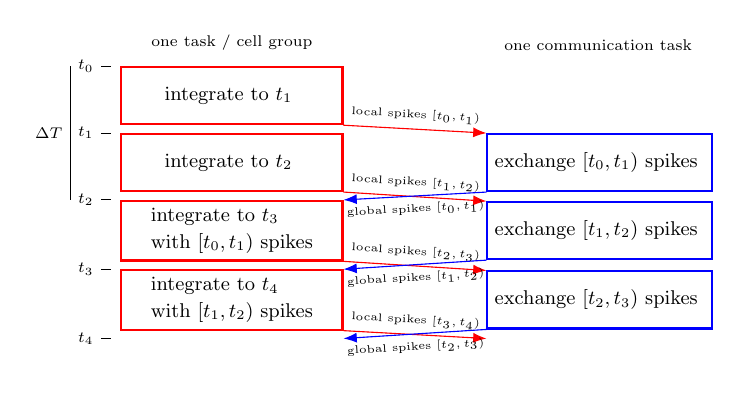
\begin{tikzpicture}
    [a/.style={rectangle, draw=red, thick, minimum height=6ex, minimum width=10em, align=left},
     b/.style={rectangle, draw=blue, thick, minimum height=6ex, minimum width=10em, align=left},
     ab/.style={-Latex, draw=red, fill=red},
     ba/.style={Latex-, draw=blue, fill=blue},
     tn/.style={minimum width=1em, align=left},
     scale=0.8, every node/.style={scale=0.8}]

    \node [a, align=left] (a0) {
    \small integrate to $t_1$
    };
    \node [a, below=1mm of a0, align=left] (a1)  {
    \small integrate to $t_2$
    };
    \node [a, below=1mm of a1] (a2) {
    \small integrate to $t_3$\\
    \small with $[t_0, t_1)$ spikes
    };
    \node [a, below=1mm of a2] (a3)  {
    \small integrate to $t_4$\\
    \small with $[t_1, t_2)$ spikes
    };
    \node [a, below=1mm of a3, minimum height=1ex, draw=none] (a4) {};

    \node [b, right=12ex of a0, draw=none] (b0) {};
    \node [b, right=12ex of a1] (b1) {
    \small exchange $[t_0,t_1)$ spikes
    };
    \node [b, right=12ex of a2] (b2) {
    \small exchange $[t_1,t_2)$ spikes
    };
    \node [b, right=12ex of a3] (b3) {
    \small exchange $[t_2,t_3)$ spikes
    };
    \node [b, right=12ex of a4, minimum height=1ex, draw=none] (b4) {};

    \draw [ab] (a0.south east) -- node [sloped, above] {\tiny local spikes $[t_0, t_1)$} (b1.north west);
    \draw [ab] (a1.south east) -- node [sloped, above] {\tiny local spikes $[t_1, t_2)$} (b2.north west);
    \draw [ab] (a2.south east) -- node [sloped, above] {\tiny local spikes $[t_2, t_3)$} (b3.north west);
    \draw [ab] (a3.south east) -- node [sloped, above] {\tiny local spikes $[t_3, t_4)$} (b4.north west);

    \draw [ba] (a2.north east) -- node [sloped, below] {\tiny global spikes $[t_0, t_1)$} (b1.south west);
    \draw [ba] (a3.north east) -- node [sloped, below] {\tiny global spikes $[t_1, t_2)$} (b2.south west);
    \draw [ba] (a4.north east) -- node [sloped, below] {\tiny global spikes $[t_2, t_3)$} (b3.south west);

    \draw ([xshift=-1ex] a0.north west) -- ++(-1ex, 0) node [tn, left] (t0) {\scriptsize $t_0$};
    \draw ([xshift=-1ex] a1.north west) -- ++(-1ex, 0) node [tn, left] {\scriptsize $t_1$};
    \draw ([xshift=-1ex] a2.north west) -- ++(-1ex, 0) node [tn, left] (t2) {\scriptsize $t_2$};
    \draw ([xshift=-1ex] a3.north west) -- ++(-1ex, 0) node [tn, left] {\scriptsize $t_3$};
    \draw ([xshift=-1ex] a4.north west) -- ++(-1ex, 0) node [tn, left] {\scriptsize $t_4$};

    \draw (t0.west) -- node [left] {\scriptsize $\Delta T$} (t2.west);

    \node [above=1mm of a0.north] {\scriptsize one task / cell group};
    \node [above=1mm of b0.north] {\scriptsize one communication task};
\end{tikzpicture}

    \label{fig:overlap}
\end{center}

Overlapping computation and communication hides latency.\\
\end{frame}
%-------------------------------------------

%-------------------------------------------
\cscschapter{3. Extensibility}
%-------------------------------------------

%-------------------------------------------
\begin{frame}[fragile]{Extensible design}
Arbor is extensible on several levels: 
\begin{enumerate}
    \item Allows new cell kinds: 
	\begin{itemize}
        \item Cable cells: morphologically detailed.
        \item LIF cells: Leaky integrate and fire point neurons.
        \item Spike source cells: Point neurons firing at a schedule.
	\end{itemize}
    \item Allows new hardware architectures and backends: 
	\begin{itemize}
        \item GPU backends: CUDA and HIP.
        \item CPU vector backends: AVX2, AVX512, Neon, SVE.
	\end{itemize}
    \item Allows new numerical implementations.
	\begin{itemize}
        \item Finite volume method. 
	\end{itemize}
\end{enumerate}

\vspace{10pt}

We can mix and match cell kind, numerical implementation and hardware backend for easy extension. 

\end{frame}
%-------------------------------------------

%-------------------------------------------
\begin{frame}[fragile]{The end}
    \arbor is under active, open, development.

    \vspace{10pt}

    \begin{center}
        \arbor is \emph{open source software}:\\
        \vspace{3pt}
        \begin{lstlisting}[style=talkpseudo]
                  github.com/arbor-sim/arbor
        \end{lstlisting}
    \end{center}

    Version 0.5.2 released June 2021.
\end{frame}
%-------------------------------------------

%-------------------------------------------
\begin{frame}[fragile]{}
    \begin{center}
        \includegraphics[height=0.15\textwidth]{logos/HBP_logo.jpg}
        \\ \vfill

        This research has received funding from the European Unions Horizon 2020 Framework Programme for Research and
        Innovation under the Specific Grant Agreement No. 720270 (Human Brain Project SGA1), Specific Grant Agreement
        No. 785907 (Human Brain Project SGA2), and Specific Grant Agreement No. 945539 (Human Brain Project SGA3).
        \\ \vfill

        \includegraphics[height=0.1\textwidth]{logos/julich_logo.pdf}
        \hspace{1cm}
        \includegraphics[height=0.09\textwidth]{logos/cscs_logo.pdf}
    \end{center}

\end{frame}
%-------------------------------------------

\end{document}
